\chapter{Diagrammi di Design}
\label{Diagrammi}

\section{Schema per la Persistenza Dati}

  \begin{figure}[H]
     \centering
     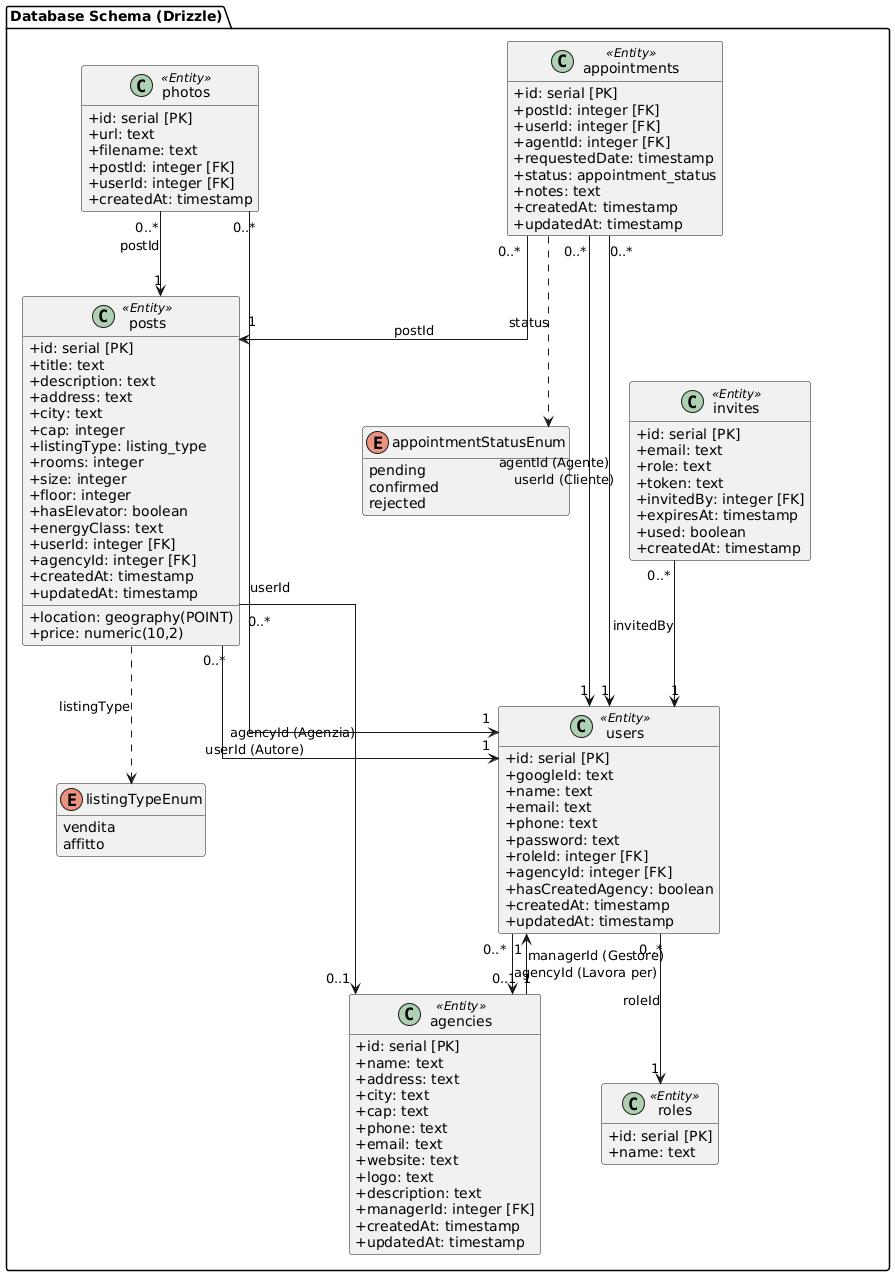
\includegraphics[width=0.8\textwidth]{images/ErUML.png}
     \caption{Diagramma ER dello Schema Dati}
     \label{fig:ER}
 \end{figure}

Lo schema dati è stato definito utilizzando Drizzle ORM (vedi \texttt{src/db/schema/}). Le tabelle principali includono \texttt{users}, \texttt{agencies}, \texttt{posts} (inserzioni), \texttt{appointments} (appuntamenti) e \texttt{invites}. Abbiamo utilizzato le capacità di Drizzle per definire relazioni (es. \texttt{one-to-many} tra agenzia e agenti) e tipi di dati specifici (es. \texttt{pgEnum} per gli stati e \texttt{customType} per i dati geografici PostGIS).


\section{Diagramma delle Classi di Design}
% Riferimento Traccia: "Diagramma delle classi di design."
% Inserisci qui il diagramma delle classi (puoi generarlo da SonarQube o modellarlo in UML)


  \subsection{Login}

  \begin{figure}[H]
     \centering
     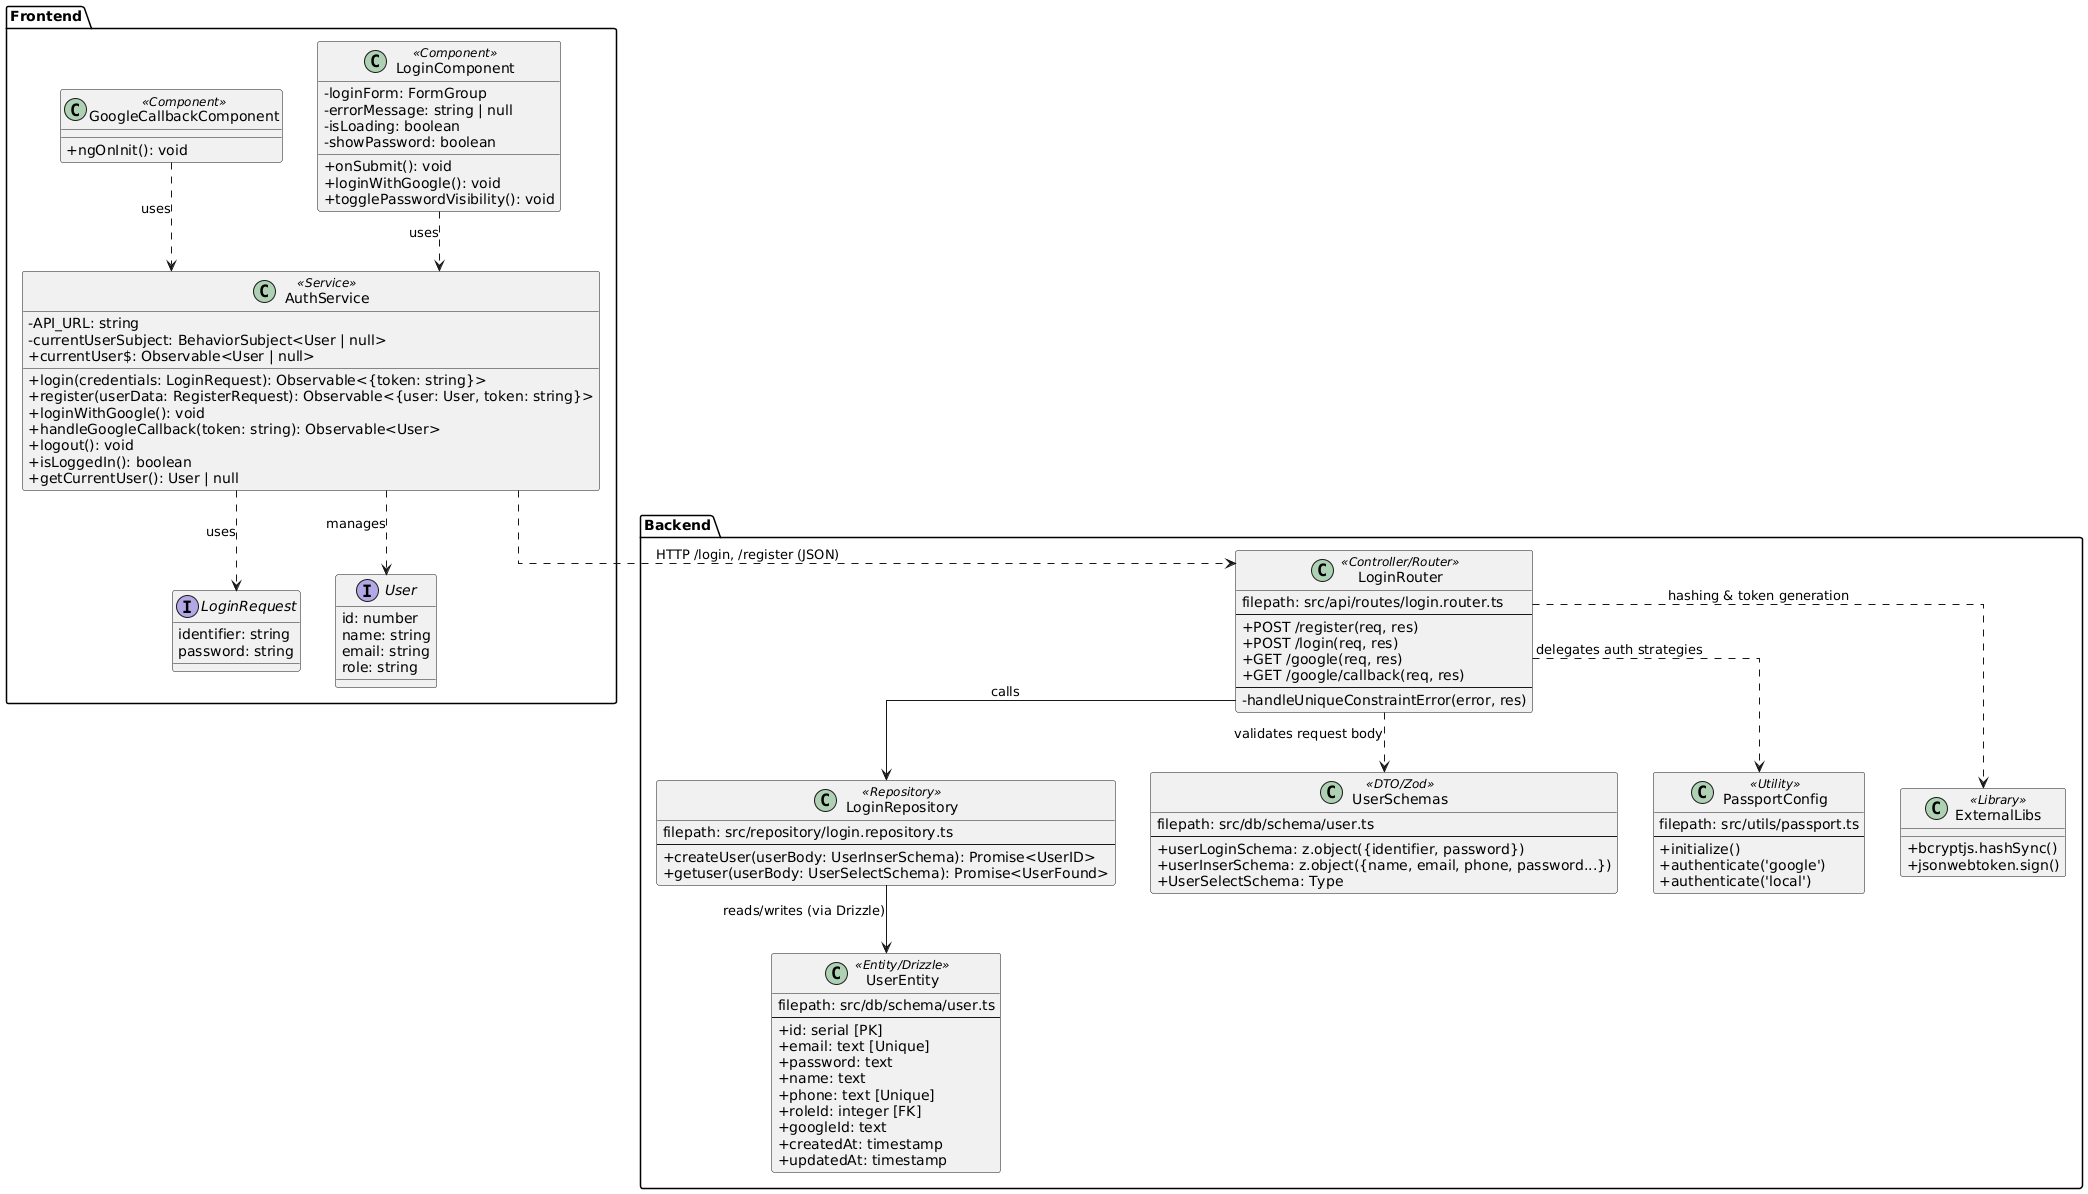
\includegraphics[width=0.8\textwidth]{images/LoginUML.png}
     \caption{Diagramma delle Classi di Design per il Login}
     \label{fig:LoginUML}
 \end{figure}

   \subsection{Registrazione Utente}

  \begin{figure}[H]
     \centering
     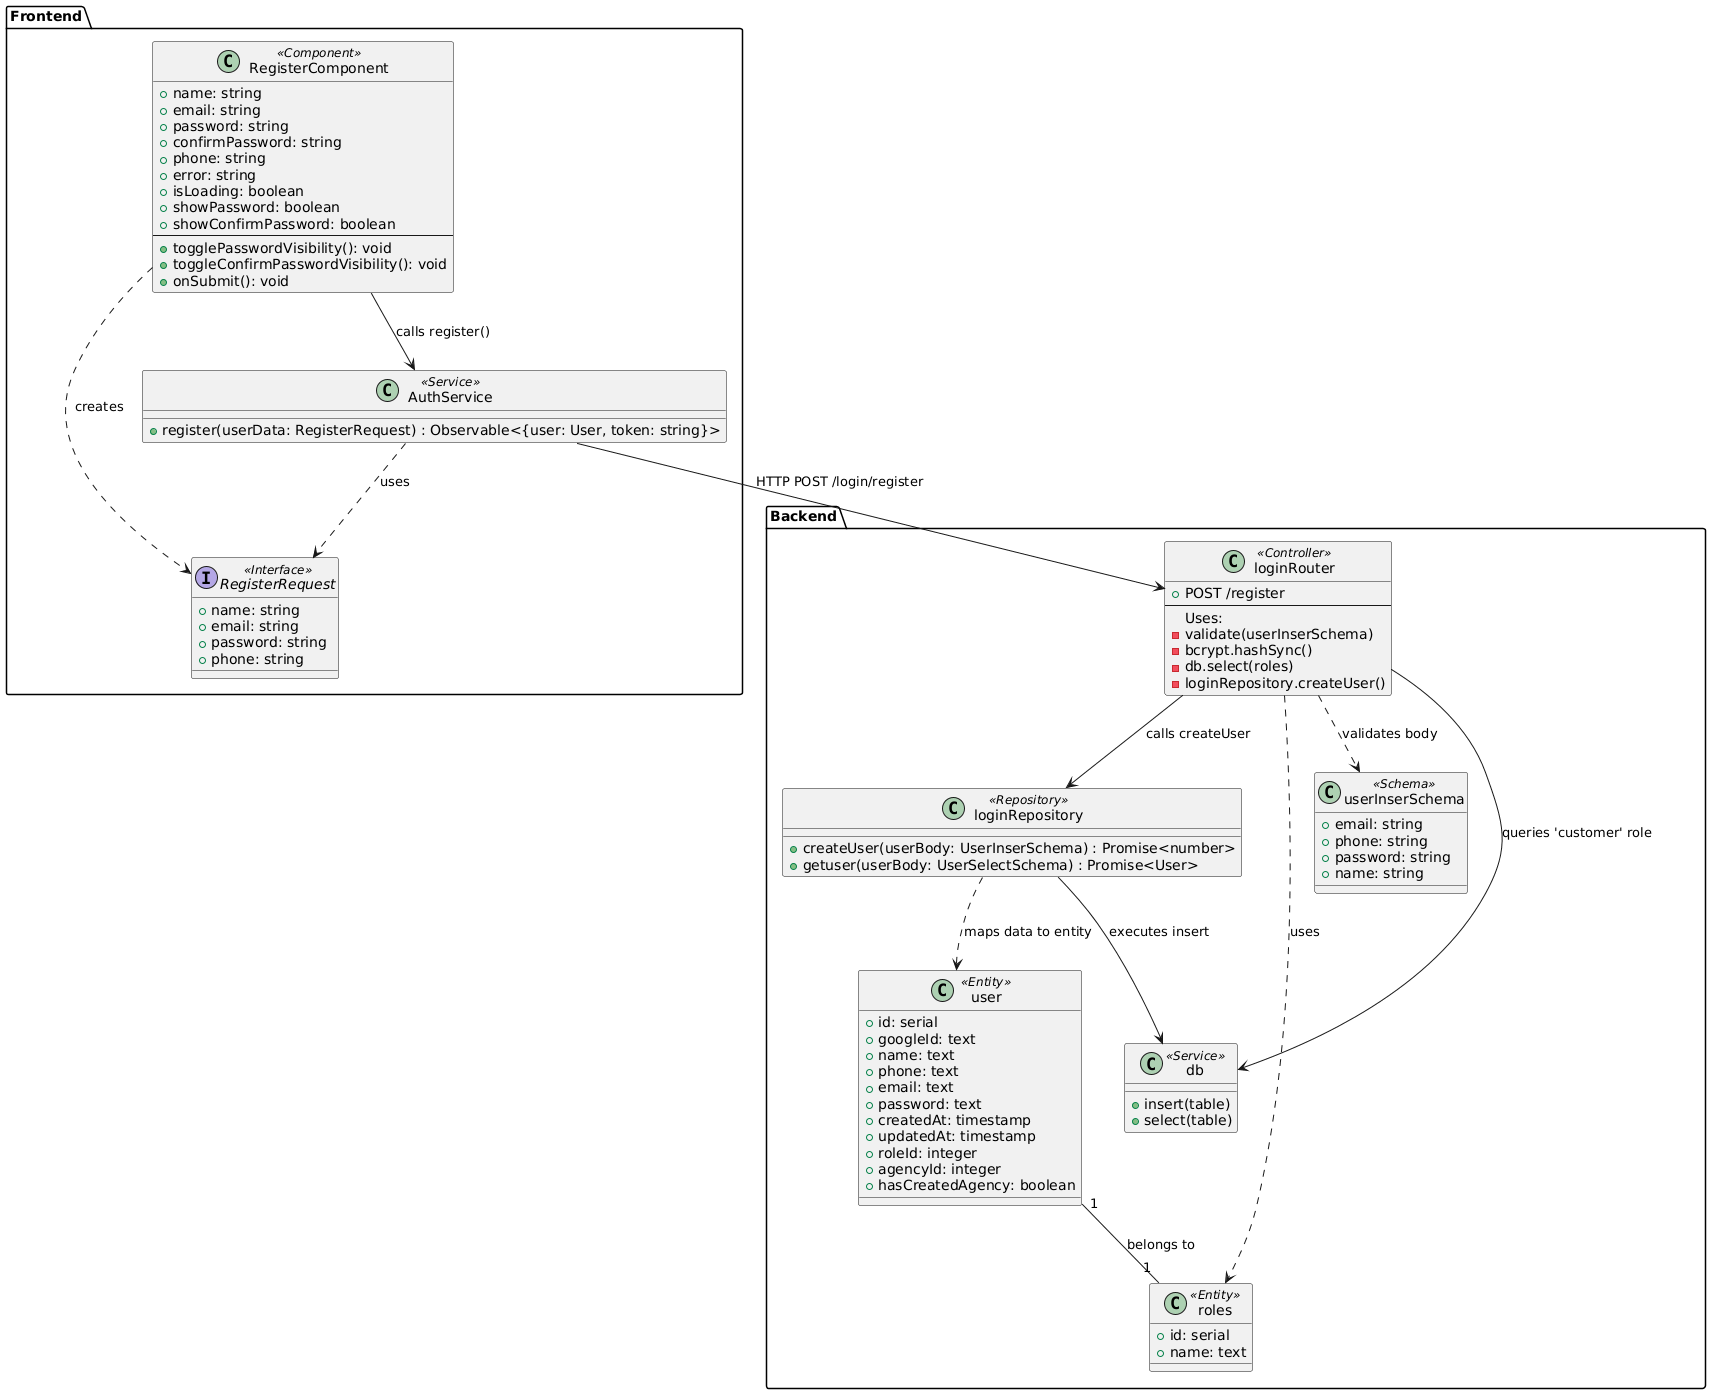
\includegraphics[width=0.8\textwidth]{images/RegisterUML.png}
     \caption{Diagramma delle Classi di Design per la Registrazione Utente}
     \label{fig:RegisterUML}
 \end{figure}

    \subsection{Cambio Password (Admin)}

  \begin{figure}[H]
     \centering
     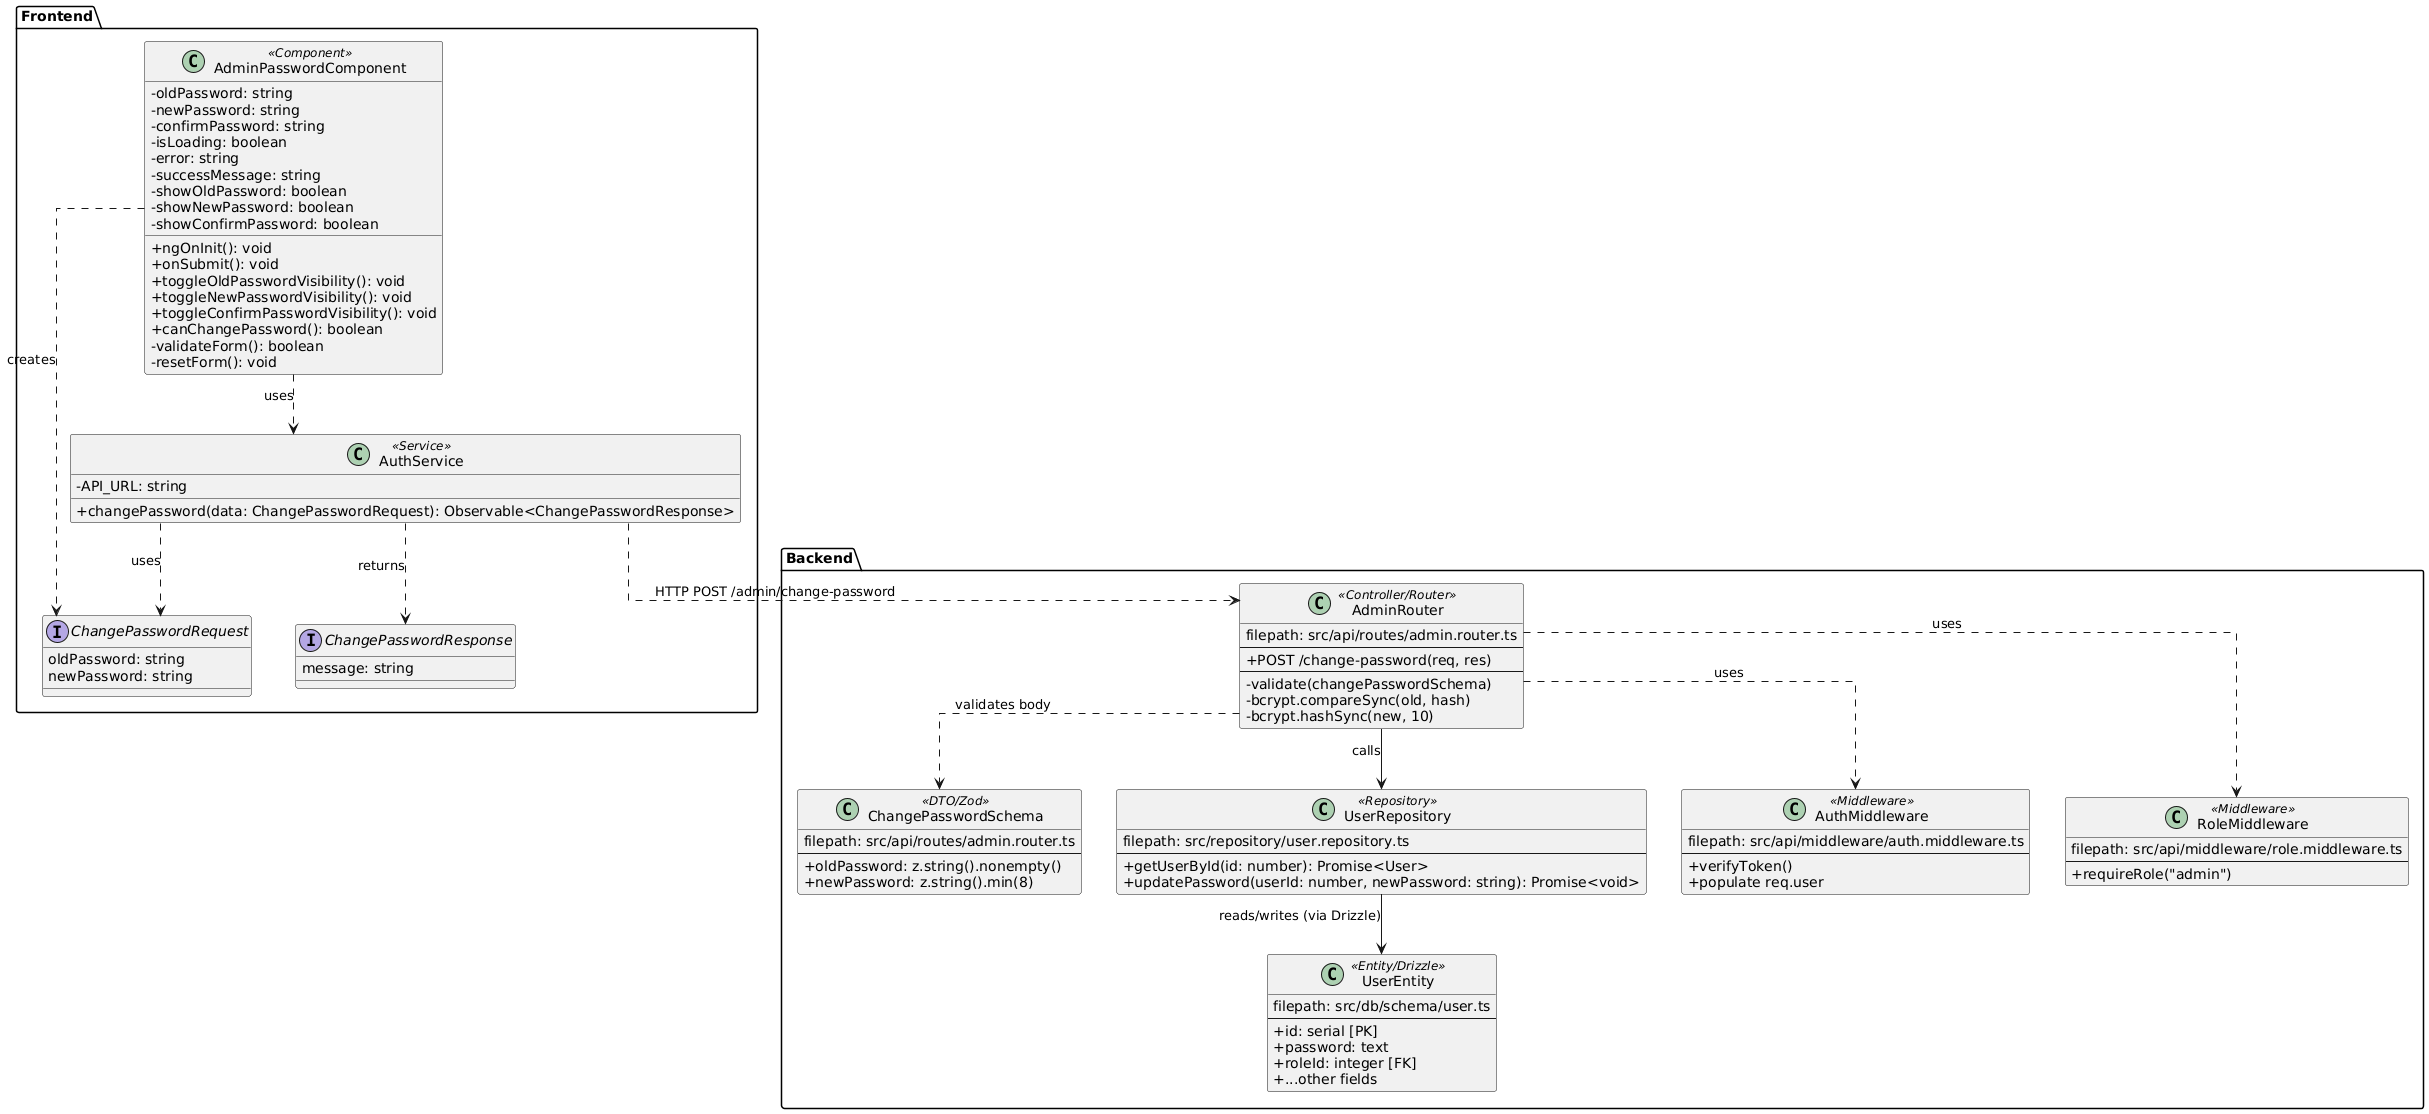
\includegraphics[width=0.8\textwidth]{images/ChangePasswordUML.png}
     \caption{Diagramma delle Classi di Design per il Cambio Password (Admin)}
     \label{fig:ChangePasswordUML}
 \end{figure}

     \subsection{Ricerca Immobile}

  \begin{figure}[H]
     \centering
     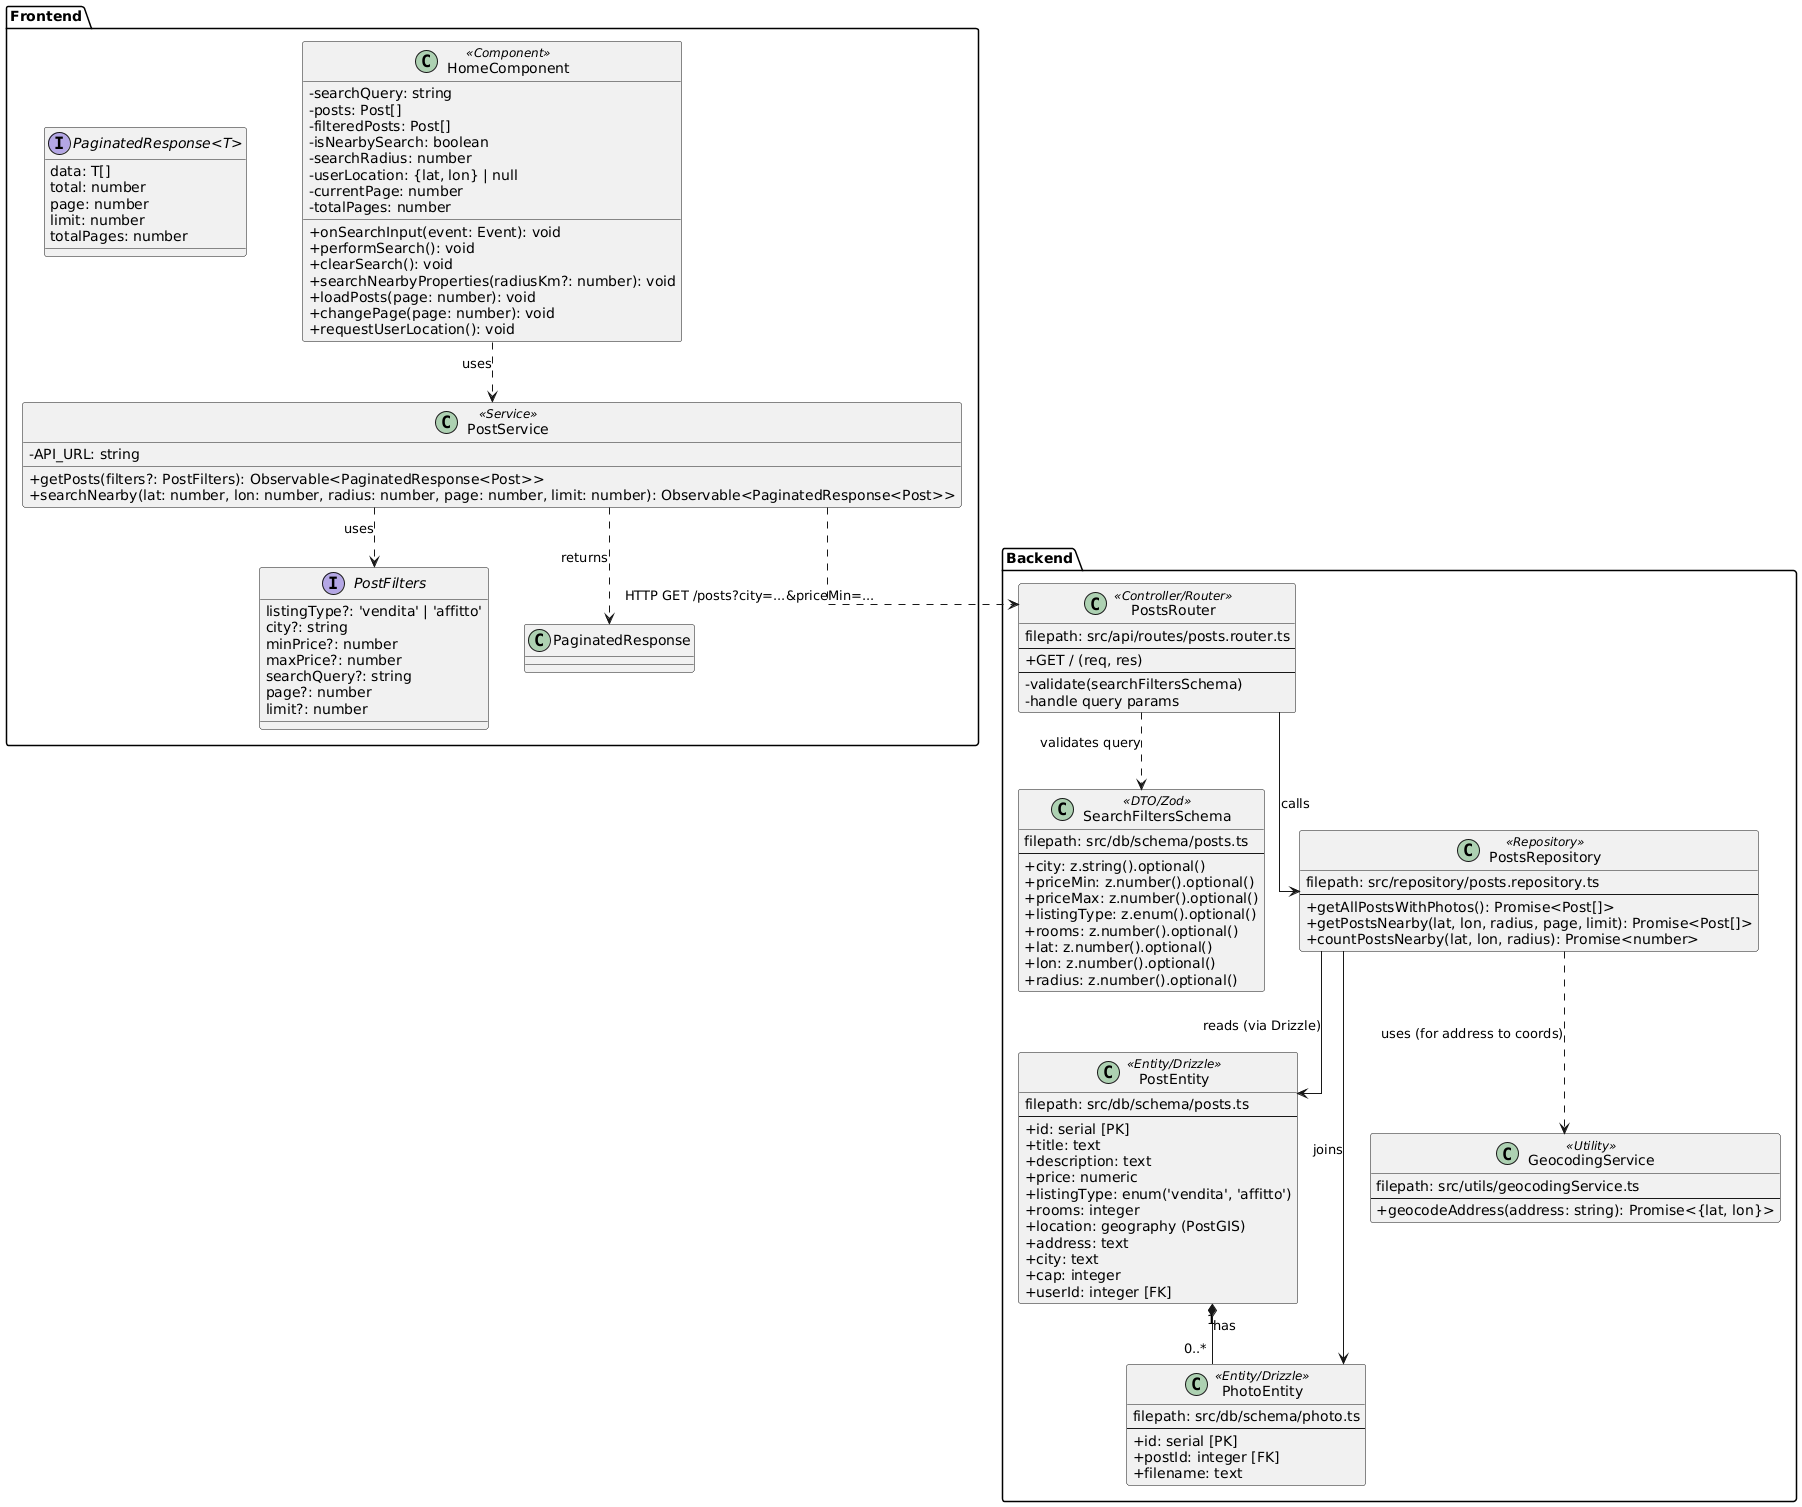
\includegraphics[width=0.8\textwidth]{images/RicercaUML.png}
     \caption{Diagramma delle Classi di Design per la Ricerca Immobile}
     \label{fig:RicercaUML}
 \end{figure}

     \subsection{Gestione Inserzioni}

  \begin{figure}[H]
     \centering
     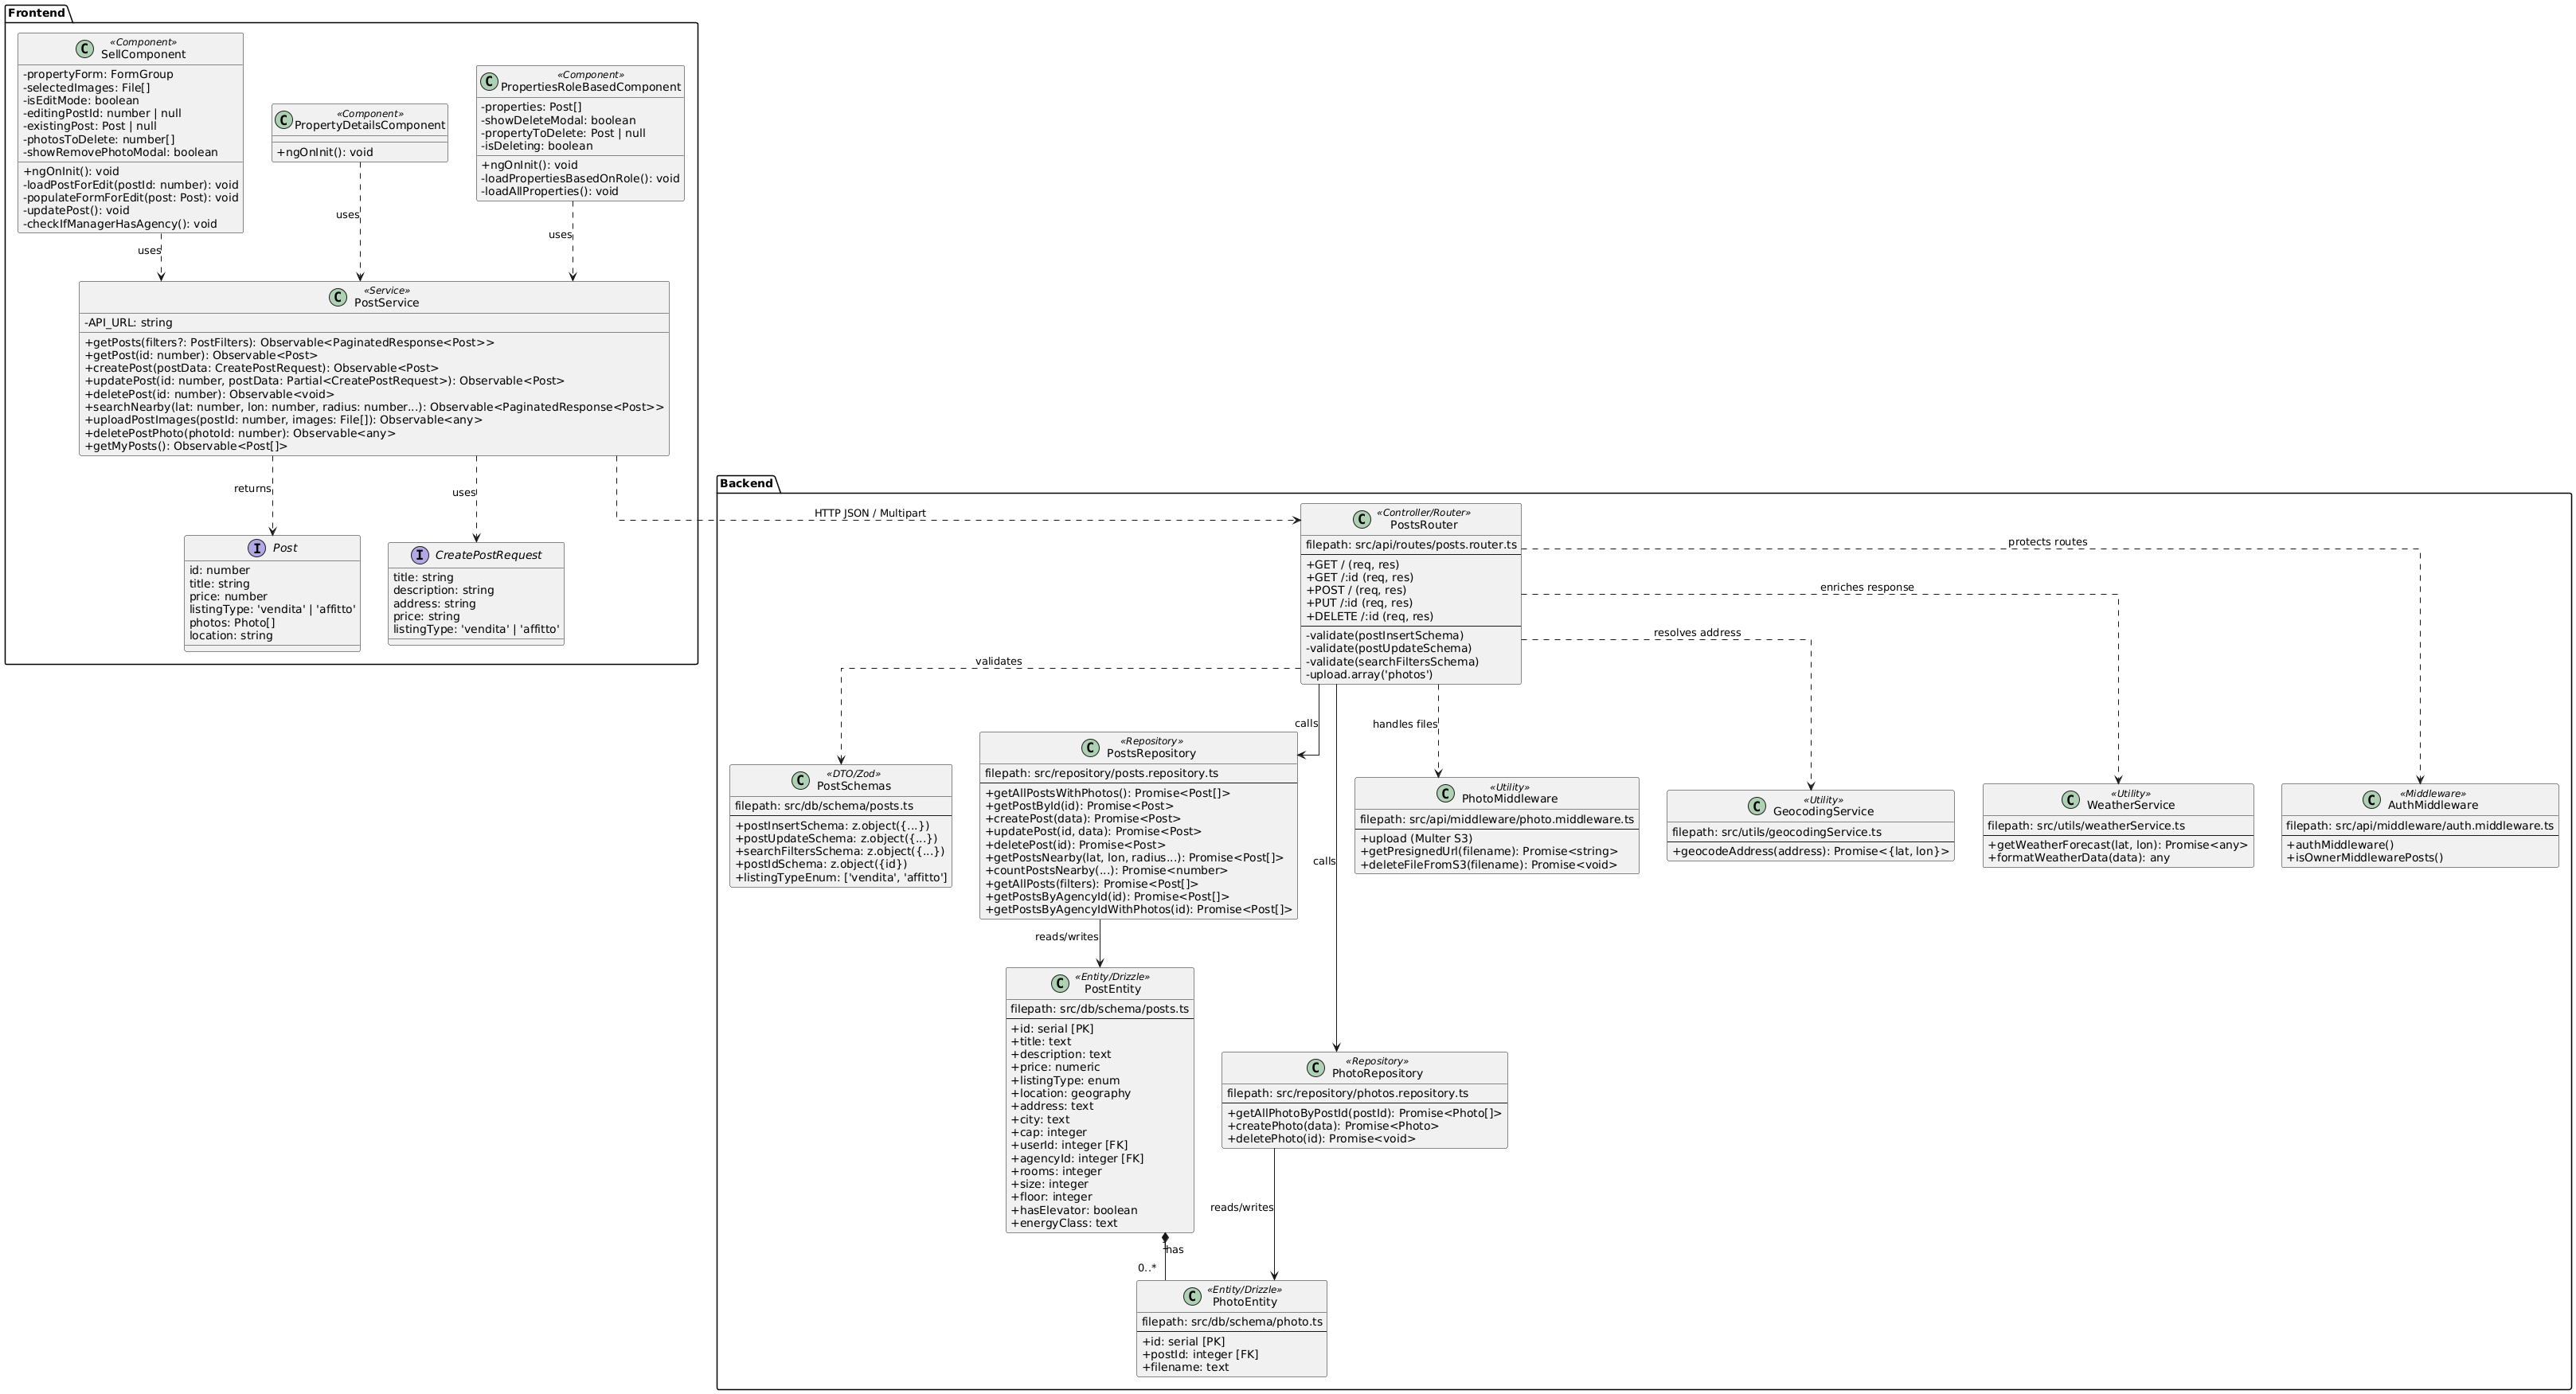
\includegraphics[width=0.8\textwidth]{images/InserzioniUML.png}
     \caption{Diagramma delle Classi di Design per la Gestione Inserzioni}
     \label{fig:InserzioniUML}
 \end{figure}

     \subsection{Gestione Appuntamenti}

  \begin{figure}[H]
     \centering
     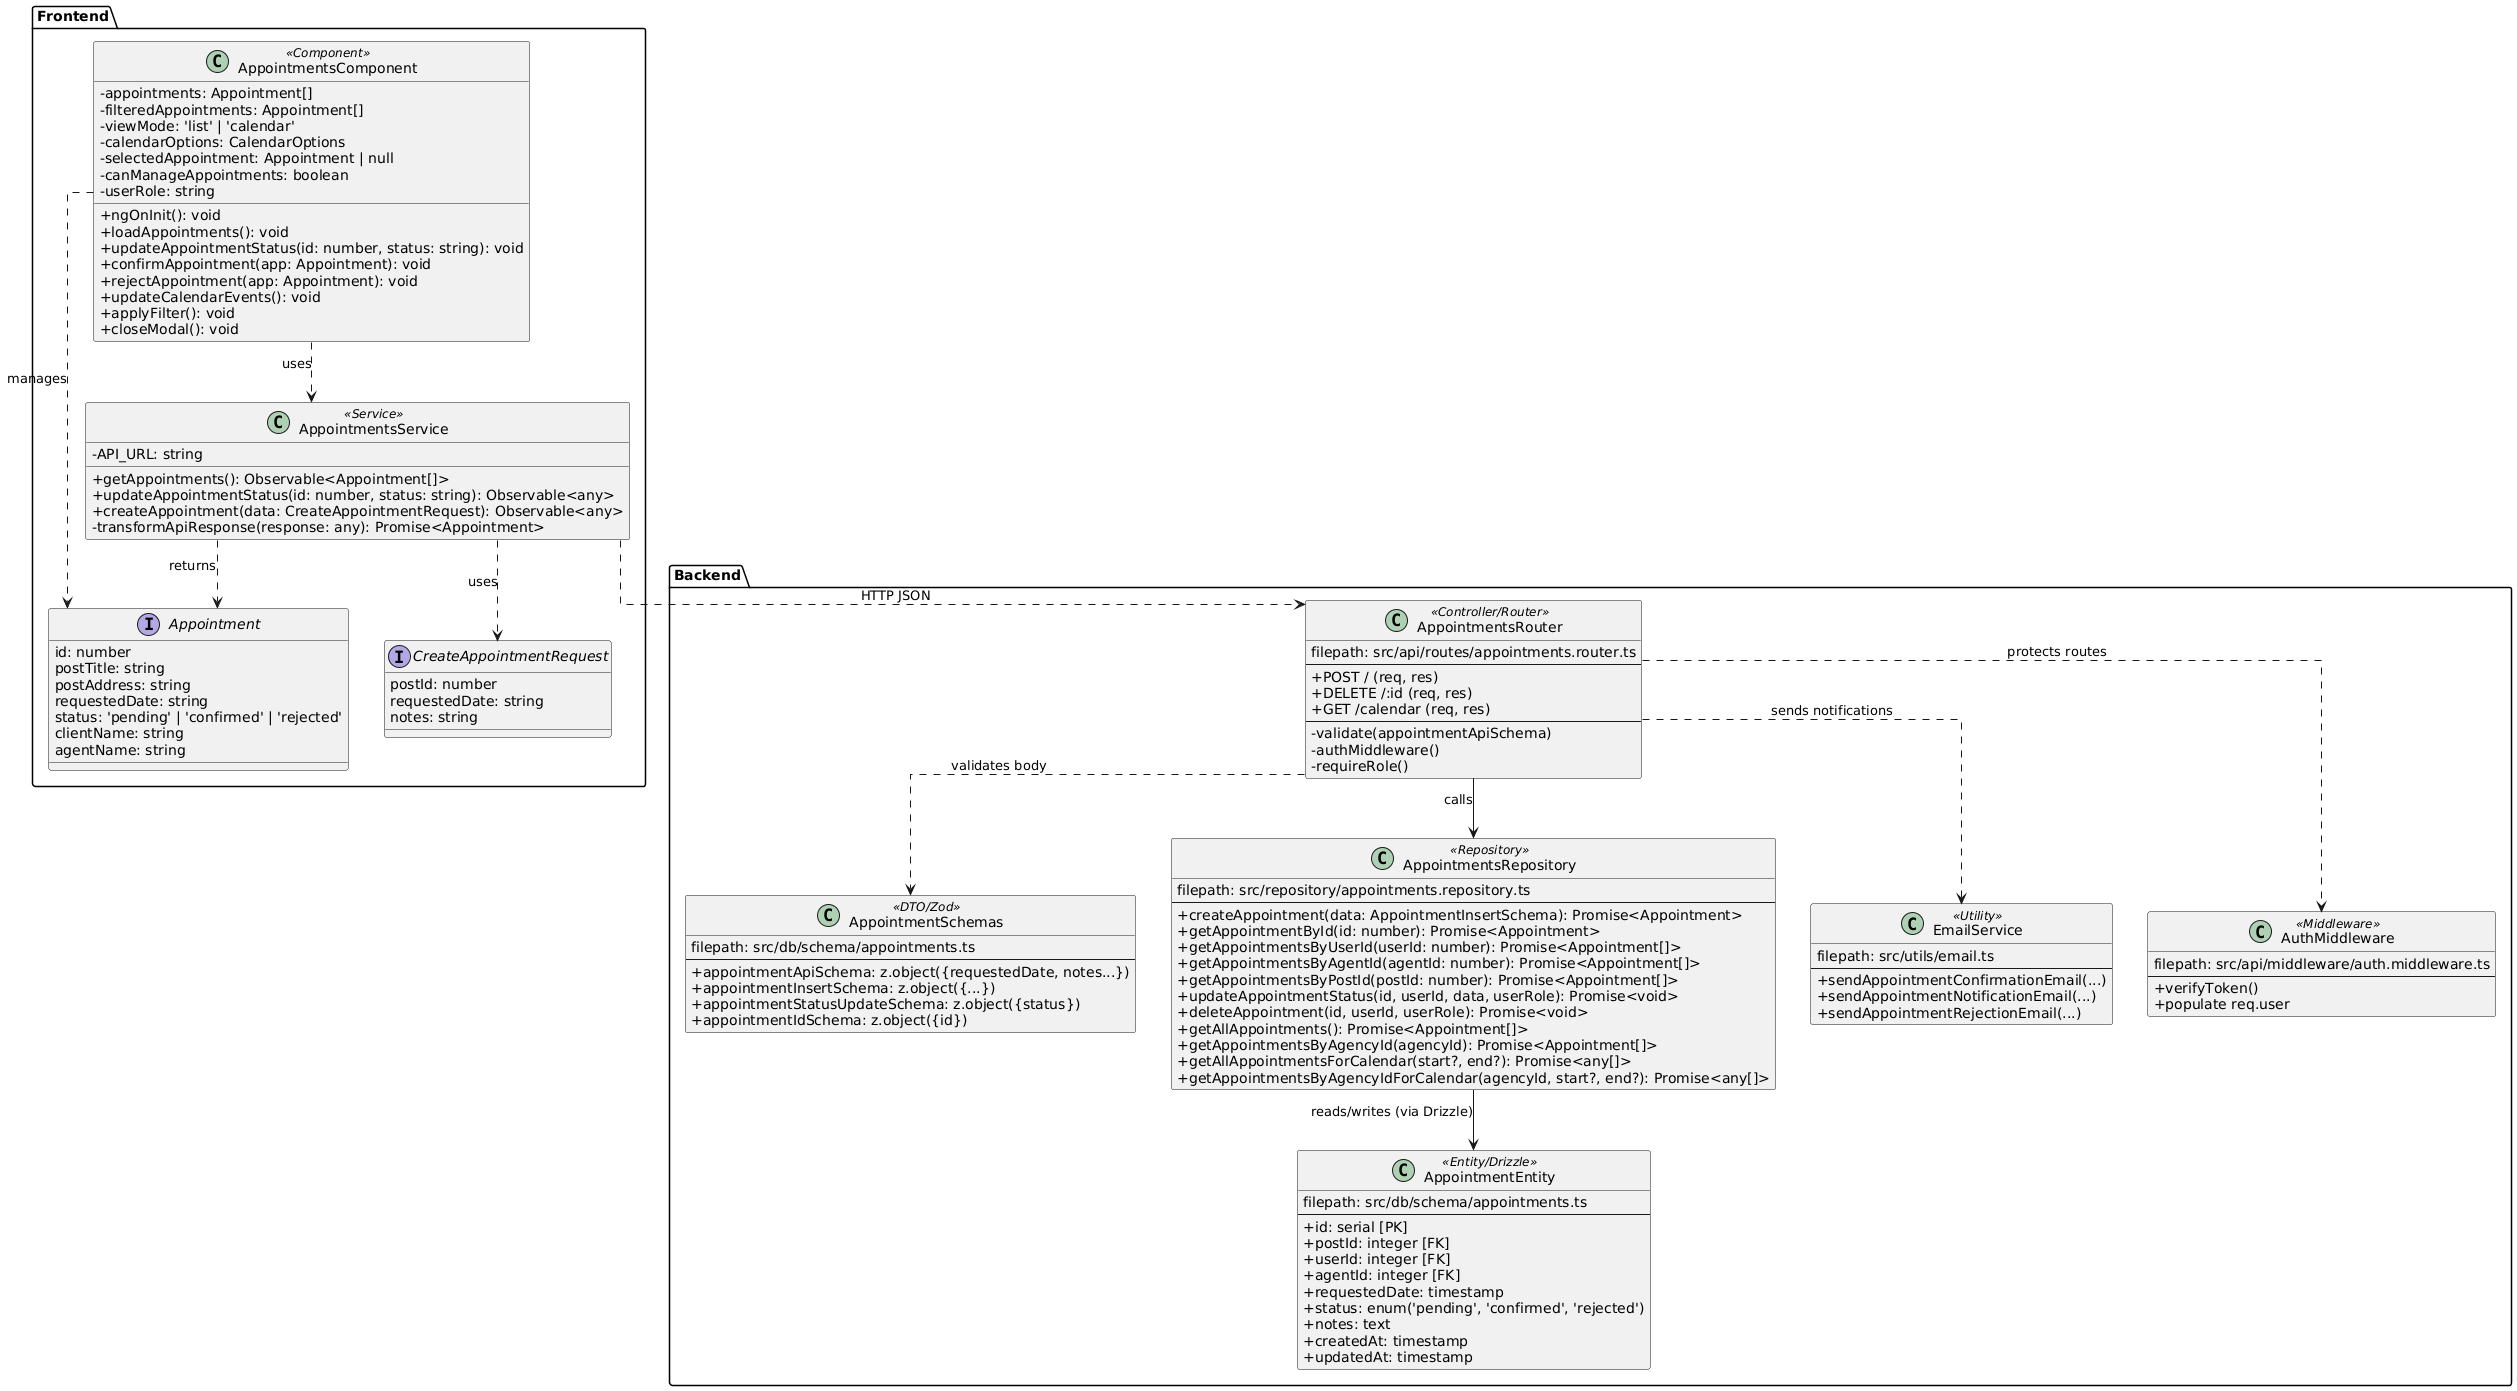
\includegraphics[width=0.8\textwidth]{images/AppuntamentiUML.png}
     \caption{Diagramma delle Classi di Design per la Gestione Appuntamenti}
     \label{fig:AppuntamentiUML}
 \end{figure}

     \subsection{Gestione Inviti}

  \begin{figure}[H]
     \centering
     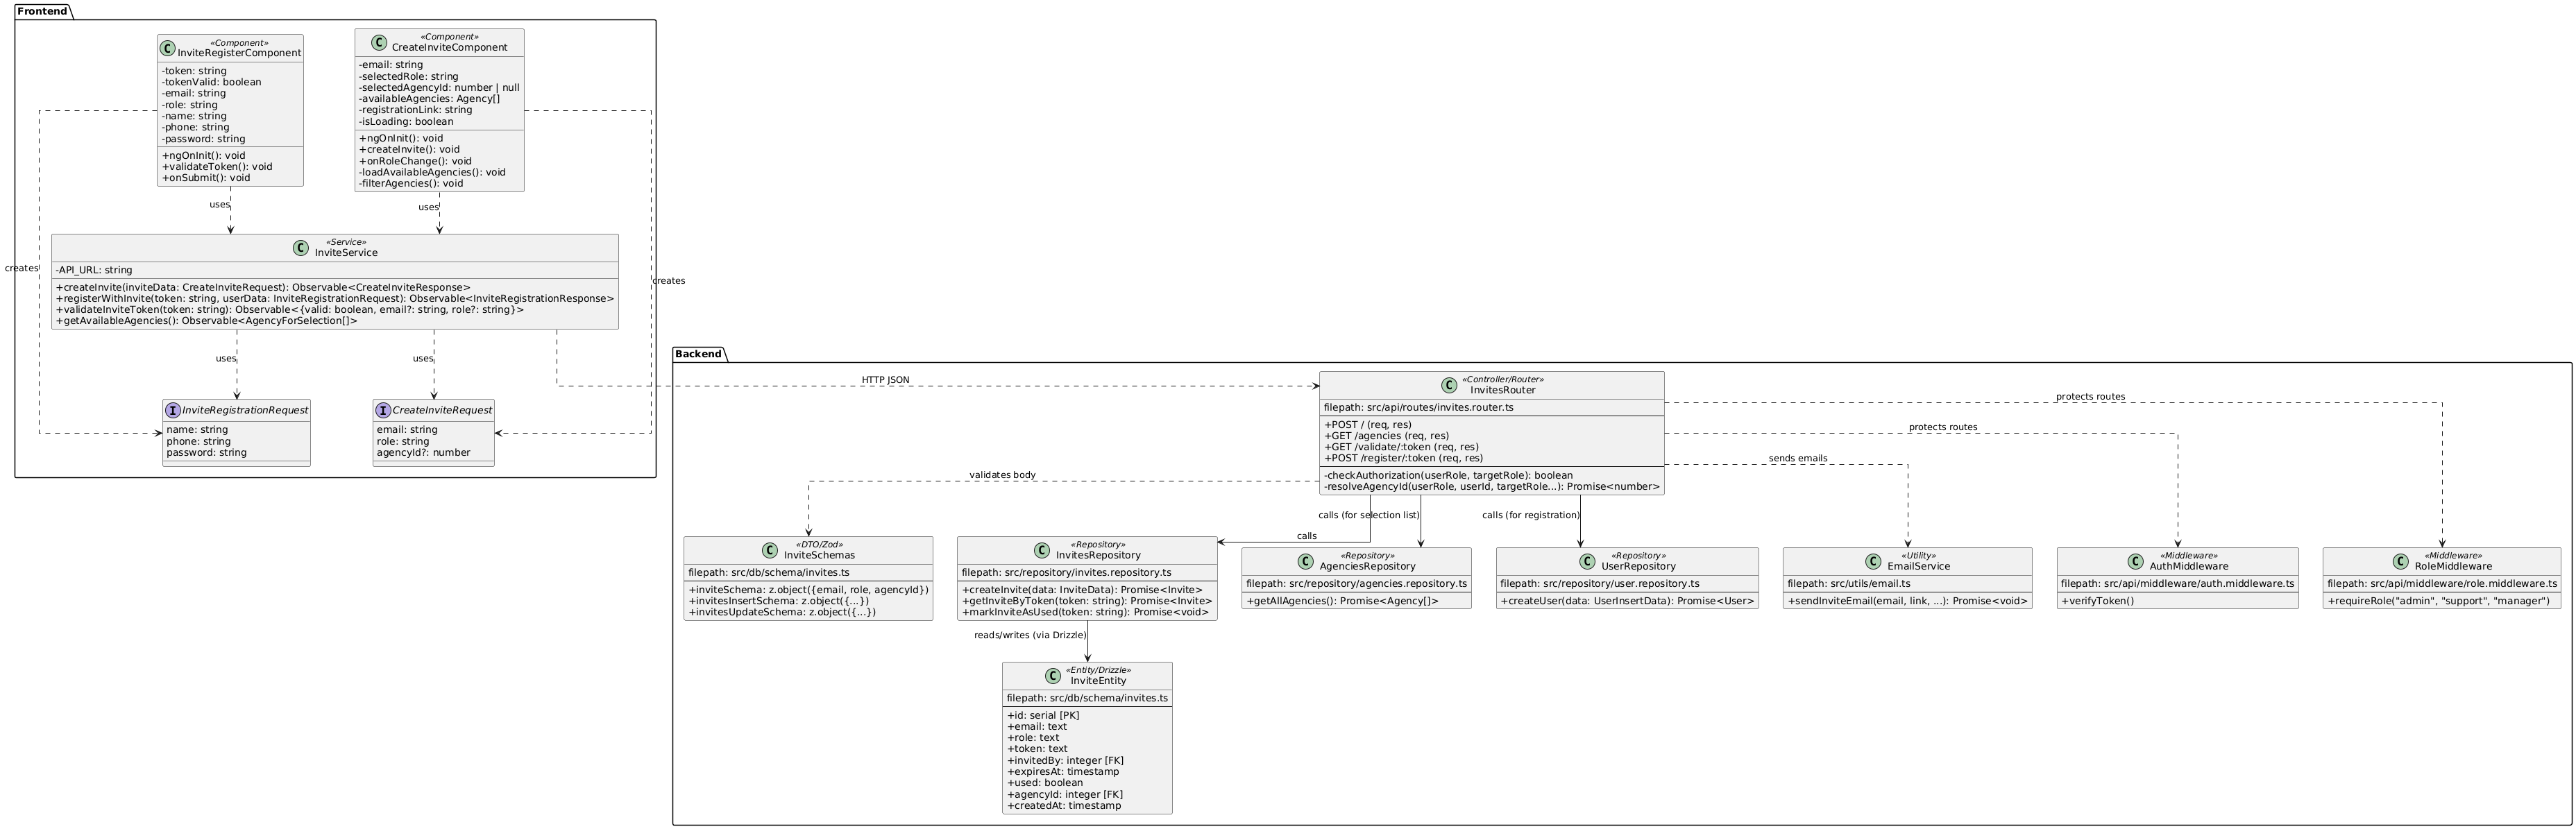
\includegraphics[width=0.8\textwidth]{images/InvitiUML.png}
     \caption{Diagramma delle Classi di Design per la Gestione Inviti}
     \label{fig:InvitiUML}
 \end{figure}

     \subsection{Gestione Agenzie}

  \begin{figure}[H]
     \centering
     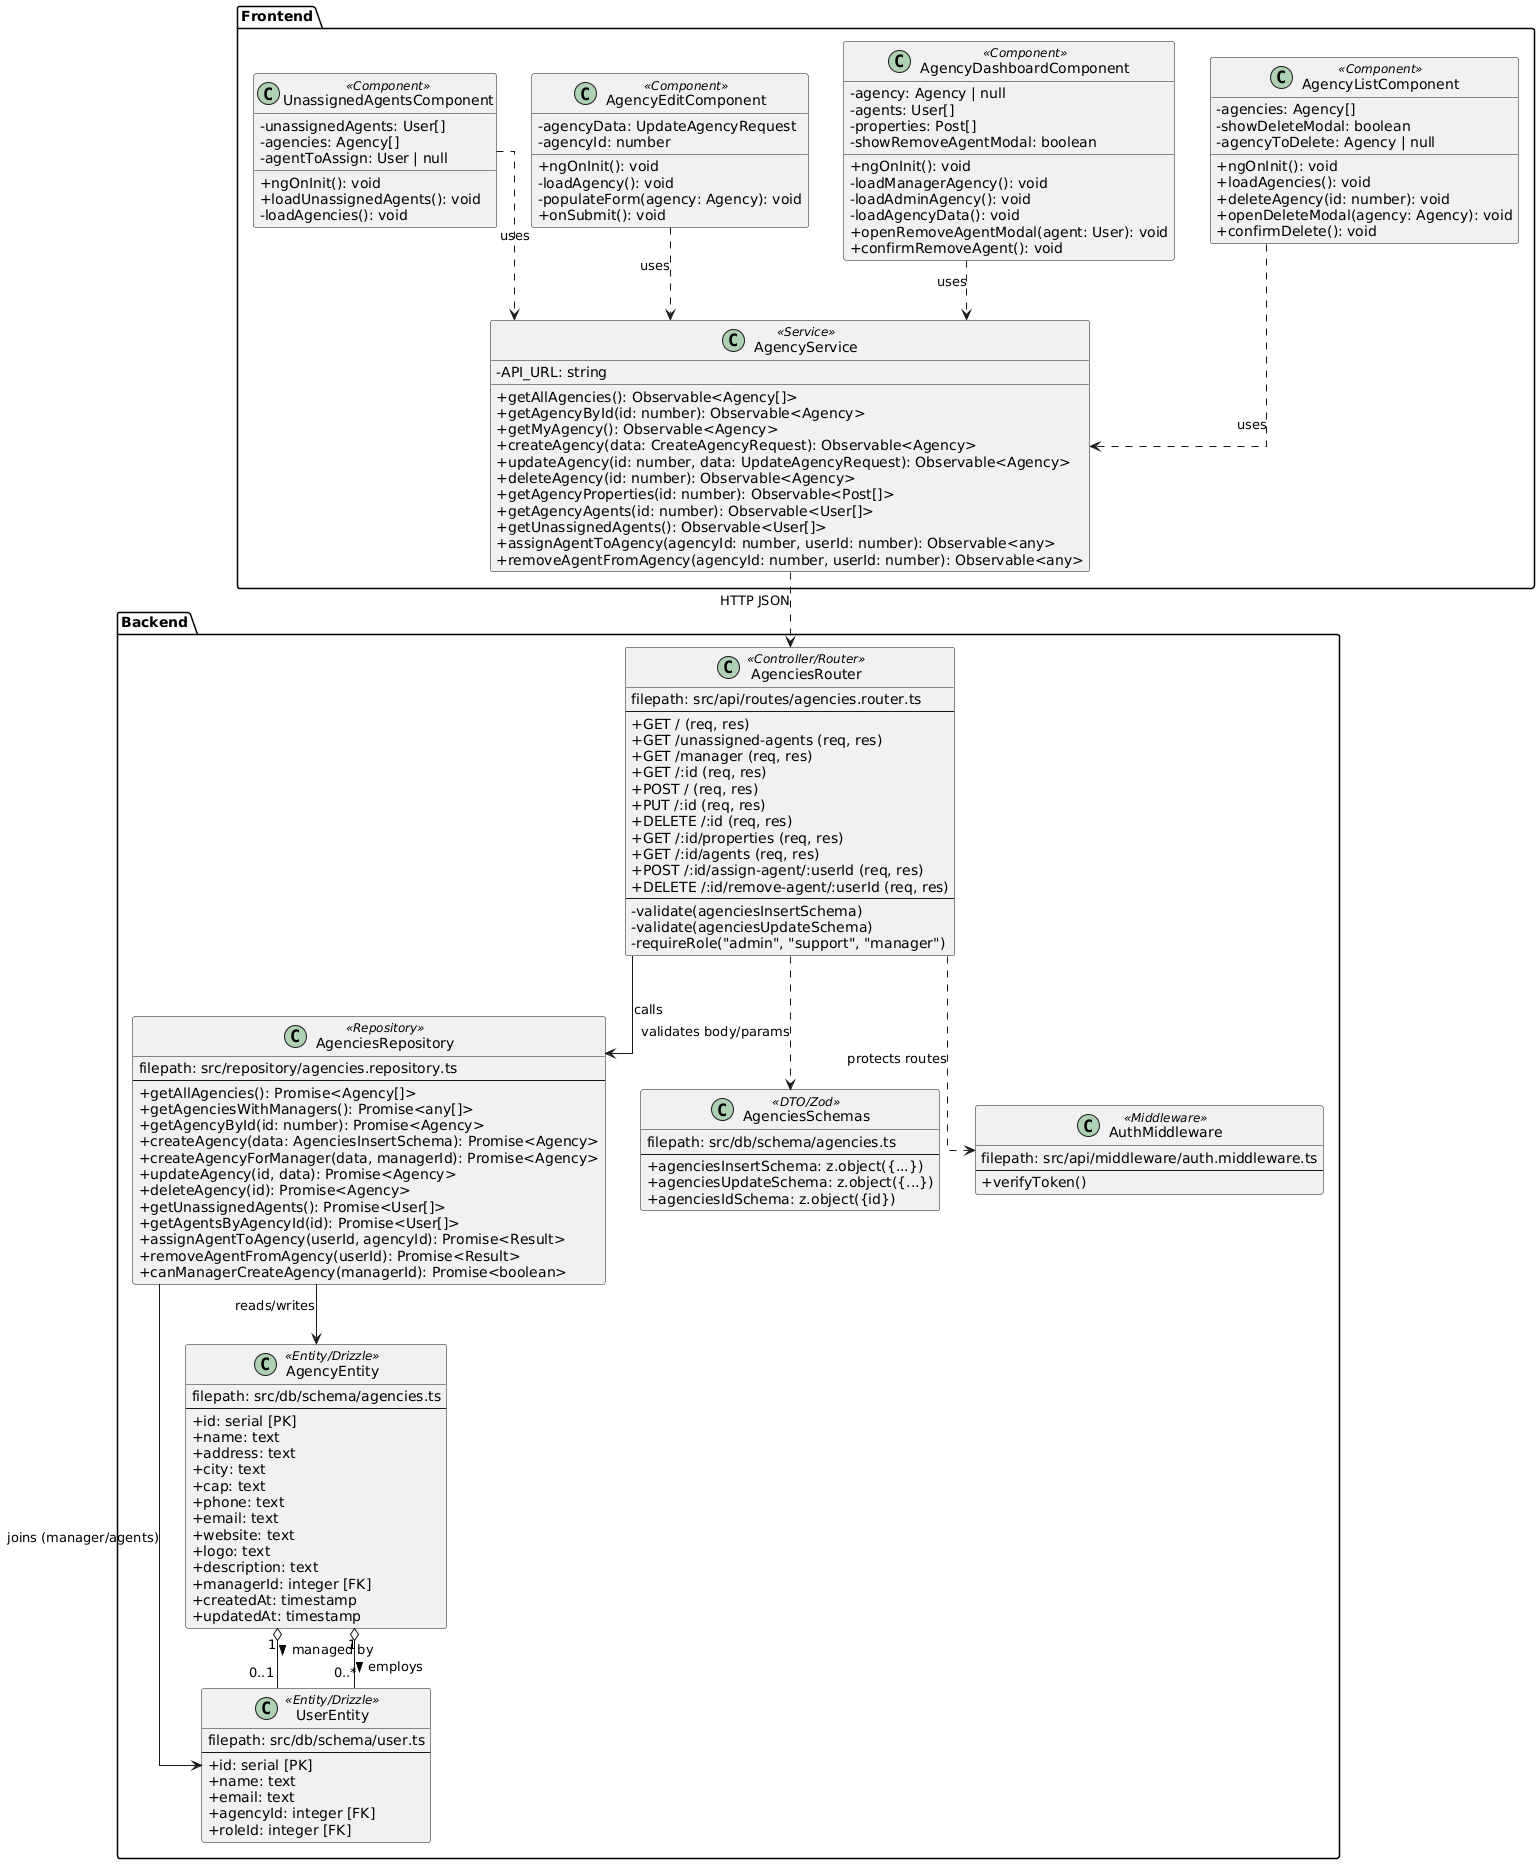
\includegraphics[width=0.8\textwidth]{images/AgenzieUML.png}
     \caption{Diagramma delle Classi di Design per la Gestione Agenzie}
     \label{fig:AgenzieUML}
 \end{figure}








\section{Diagrammi di Sequenza di Design}
% Riferimento Traccia: "Diagrammi di sequenza di design per i casi d'uso..."
% Inserisci qui i diagrammi di sequenza per i 4 casi d'uso scelti.
\textit{[Placeholder per i Diagrammi di Sequenza UML (es. Prenotazione Visita, Ricerca Immobile, etc.).]}



% =====================================================================

